\documentclass{article}
\usepackage{amsmath}
\usepackage{graphicx,xcolor}
\usepackage{wrapfig}
\usepackage[margin=1in]{geometry}
\usepackage[square,numbers]{natbib}
\bibliographystyle{unsrt}

	

\begin{document}
\centerline{
\large
Dynamic Information Extraction and Provenance Ledger for Edge AI
}
\normalsize
	\noindent\textbf{PI Ryan Coffee} -- Sr. Staff Scientist, LCLS/PULSE, SLAC National Accelerator Laboratory, \\coffee@slac.stanford.edu, 650-387-0981, \\
	Audrey Corbeil Therrien -- Banting Research Fellow \& Linac Coherent Light Source (LCLS) Data Systems,\\
	Angelo Dragone -- Department Head, Integrated Circuits, Technology \& Innovation Directorate, Advanced Instrumentation For Research Division,\\
	Matt Feldman -- Graduate Fellow, Stanford Computer Science \& Developer SambaNova Systems, \\
	Ryan Herbst -- Department Head, Electronics Systems, Technology \& Innovation Directorate, Advanced Instrumentation For Research Division,\\
	Omar Quijano -- Department Head, Linac Coherent Light Source (LCLS) IT/Networking,\\
	Ben Taylor -- Founder and CEO, LedgerDomain, LLC.,\\
	Jana Thayer -- Department Head, Linac Coherent Light Source (LCLS) Data Systems.\\
	Topic: 1b. Advanced Scientific Computing Research -- In Situ Data Management ASCR-ISDM\\
	February 29, 2020\\

\break
\centerline{\large{Dynamic Information Extraction and Provenance Ledger for Edge AI}}
\normalsize
\vspace{0.5\baselineskip}
\centerline{\textbf{PI Ryan Coffee},
Audrey Corbeil Therrien,
Angelo Dragone,
Matt Feldman,}
\centerline{
Ryan Herbst,
Omar Quijano,
Ben Taylor, and 
Jana Thayer.
}
\centerline{February 29, 2020}
\vspace{0.5\baselineskip}

\begin{wrapfigure}[23]{r}{.4\linewidth}
	\vspace{-1.5\baselineskip}
	\centerline{ \includegraphics[clip,trim={-2cm -2cm 1.5cm 1.5cm},width=\linewidth]{./figs/plotting.technology.eps} }
	\vspace{-1\baselineskip}
	\caption{
		\label{fig::technology} 
		Adapted from Ref.~\cite{MicroprocessorTrendData}. Note that the limitations in the mid-2000s triggered the multi-threading paradigm.
	}
\end{wrapfigure}
The Linac Coherent Light Source II (LCLS-II) holds great promise to answer critical questions regarding ultra-fast materials dynamics, the molecular motion responsible for light harvesting, and the first trigger events in catalysis. 
The corresponding newly enabled experimental techniques such as femtosecond x-ray Fourier holography \cite{Tais2018}, time-domain ghost imaging \cite{Taran2020}, time-domain phonon dynamics \cite{Mariano2013,Abbamonte2013} and femtosecond resolved dark field x-ray microscopy \cite{Simons2015} extract valuable information only after sorting or otherwise statistically treating signal dependence on stochastic source parameters, e.g. time-delay, spectral content, or spatial mode.
The need to identify both very weak and/or very rare events in overwhelmingly cluttered and noisy data requires extreme data rate detectors that could be capable of one million readout frames per second either as next-generation commercial visible cameras or SLAC's own ePix family of x-ray imaging detectors. 
The raw data volume for such rates (TB/s) would be equivalent to producing 100 years worth of Ultra-HD video \cite{HowBigVideo} every day which would require nearly \$1M in new storage for each day of operation \cite{CostPerTB}.
\footnote{This only considers hardware costs. Actual costs including power, space and personnel are much higher (estimated at \$30 per GB per month) and accumulate over time.} 
Although the scale of the data for the complementary facilities LCLS-II and the upcoming Advanced Photon Source Upgrade (APS-U) pose extreme scale challenges, the evolution of 5G networked sensors driving autonomous industrial decision portends a critical need for data handling at the point of generation, at the sensor \cite{Gartner2018,NetworkWorld2019}---conventional data center hosted mining is not a viable option for DOE labs and for Industry 4.0 alike.
Similar to the multi-threading paradigm shift of the mid-2000s (Fig.~\ref{fig::technology}), the Edge AI paradigm shift is upon us now.

A significant portion of human sensory processing occurs in the sensory organs themselves such as the edge detection in the retinal ganglion cells and rapid eye stabilization.
We propose a similar function for our scientific sensors; a processing unit at the detector--Edge AI--that can analyze incoming data in real-time and provide actionable information back to the detector, out to the source, and forward to the downstream analysis networks.
These inference engines will host dynamically adaptive algorithms based on user-trained machine learned inference models that are unique to the particular scientific question and extract contextually relevant information before passage down the analysis chain.
This Edge AI system will be hosted on sensor-based Field Programmable Gate Arrays (FPGAs) and emerging flexible ``batch size=1'' inference accelerators \cite{edgetpu_benchmarks,edgetpu,waveCGRA,CGRAreview,seaofcores} that will minimize latency to alleviate the need for inappropriately large memory buffers.

The streaming information extraction must flexibly handle the weekly re-definition of actionable information since new users mount experiments with vastly different objectives every week; this precludes a static data acquisition system. 
We therefore require user trained real-time streaming inference that can dynamically route data flow through the entire acquisition chain.
The path of the data flow will typically depend on the particulars of the stochastically varying source parameters.
For instance, in the case of time-domain phonon dynamics \cite{Mariano2013}, diffuse scattering images would be sorted into time ordered bins until each bin holds sufficient statistics.
At this point the time axis would be Fourier transformed to obtain a phonon-frequency map relevant for the experiment.
Since only narrow regions in the frequency domain need to be sent from the Edge node to permanent storage, the desirable information can be as small as $10^{-3}$ compressed relative to the millions of individual images that were produce that information.
In the case of time-domain ghost imaging \cite{Taran2020}, the spectroscopic information comes from the batch covariance of measured signal with incoming x-ray pulse time-energy distribution, itself the result of a trained inference model \cite{Audrey}.
Since each group will train its own data processing and diagnostic inference models, these models will change weekly with each new arriving user group.
This weekly re-definition requires that an Edge AI system fundamentally records both data and model provenance into a transaction ledger.

The transaction ledger will log the precise actions taken on the particular data event into a unique data provenance record (see Fig.~\ref{fig::EdgeFlow}).
The ledger then will continue to track and update a quantifiable metric according to the derived scientific value of both data and algorithm.
This ``value aware'' ledger can then be used for an automated dynamic retention policy whereby lifetime in archive would scale proportionally with the evolving scientific value.
In other words, the more that data individuals or ML models are used for publications and even training subsequent inference models or the higher the impact of resulting products, the longer the data or model will remain active and discoverable in a data sharing marketplace. 
Aggregation would reveal the integrated value for scientific facilities, experimental techniques, and sensor technologies based on this quantifiable impact.
The transaction ledger can also be used to track data individuals and models given the possibility for changing levels of sensitivity and privacy that are sure to arise in any future data marketplace. 
This ability to handle varying levels of sensitivity concern is why we target a blockchain solution to data and model identification and provenance ledger.

The immediacy of our need for ultra-low latency and dynamic handling data coupled with our long history of detector development--from sensor to readout electronics to complex data pipeline design--makes SLAC a unique environment with the necessary infrastructure to develop Edge AI infrastructure.
%The LCLS-II Data System has both offline systems and a data reduction layer for near real-time processing hosted in FPGA hardware as a co-processor within the real-time processing layer or as stand-alone analysis accelerators. 
SLAC has experts in scientific instrumentation, data analysis, FPGA development, and machine learning all on-site to create, implement, and deploy the Edge AI system.
The PI will leverage his collaboration with blockchain industry partner LedgerDomain \cite{LedgerDomain,BruinChain} as well as his inter-lab and inter-agency collaborations to ensure that the developed infrastructure is compatible with an emerging data marketplace and can adapt to varying levels of open or restricted access and data redaction.
Furthermore, the PIs has existing collaboration with emerging Edge AI inference chip makers in the private sector and therefore is well positioned to develop a broadly compatible framework across DOE and Industry 4.0 at large.

\begin{figure}
	\vspace{-1\baselineskip}
	\centerline{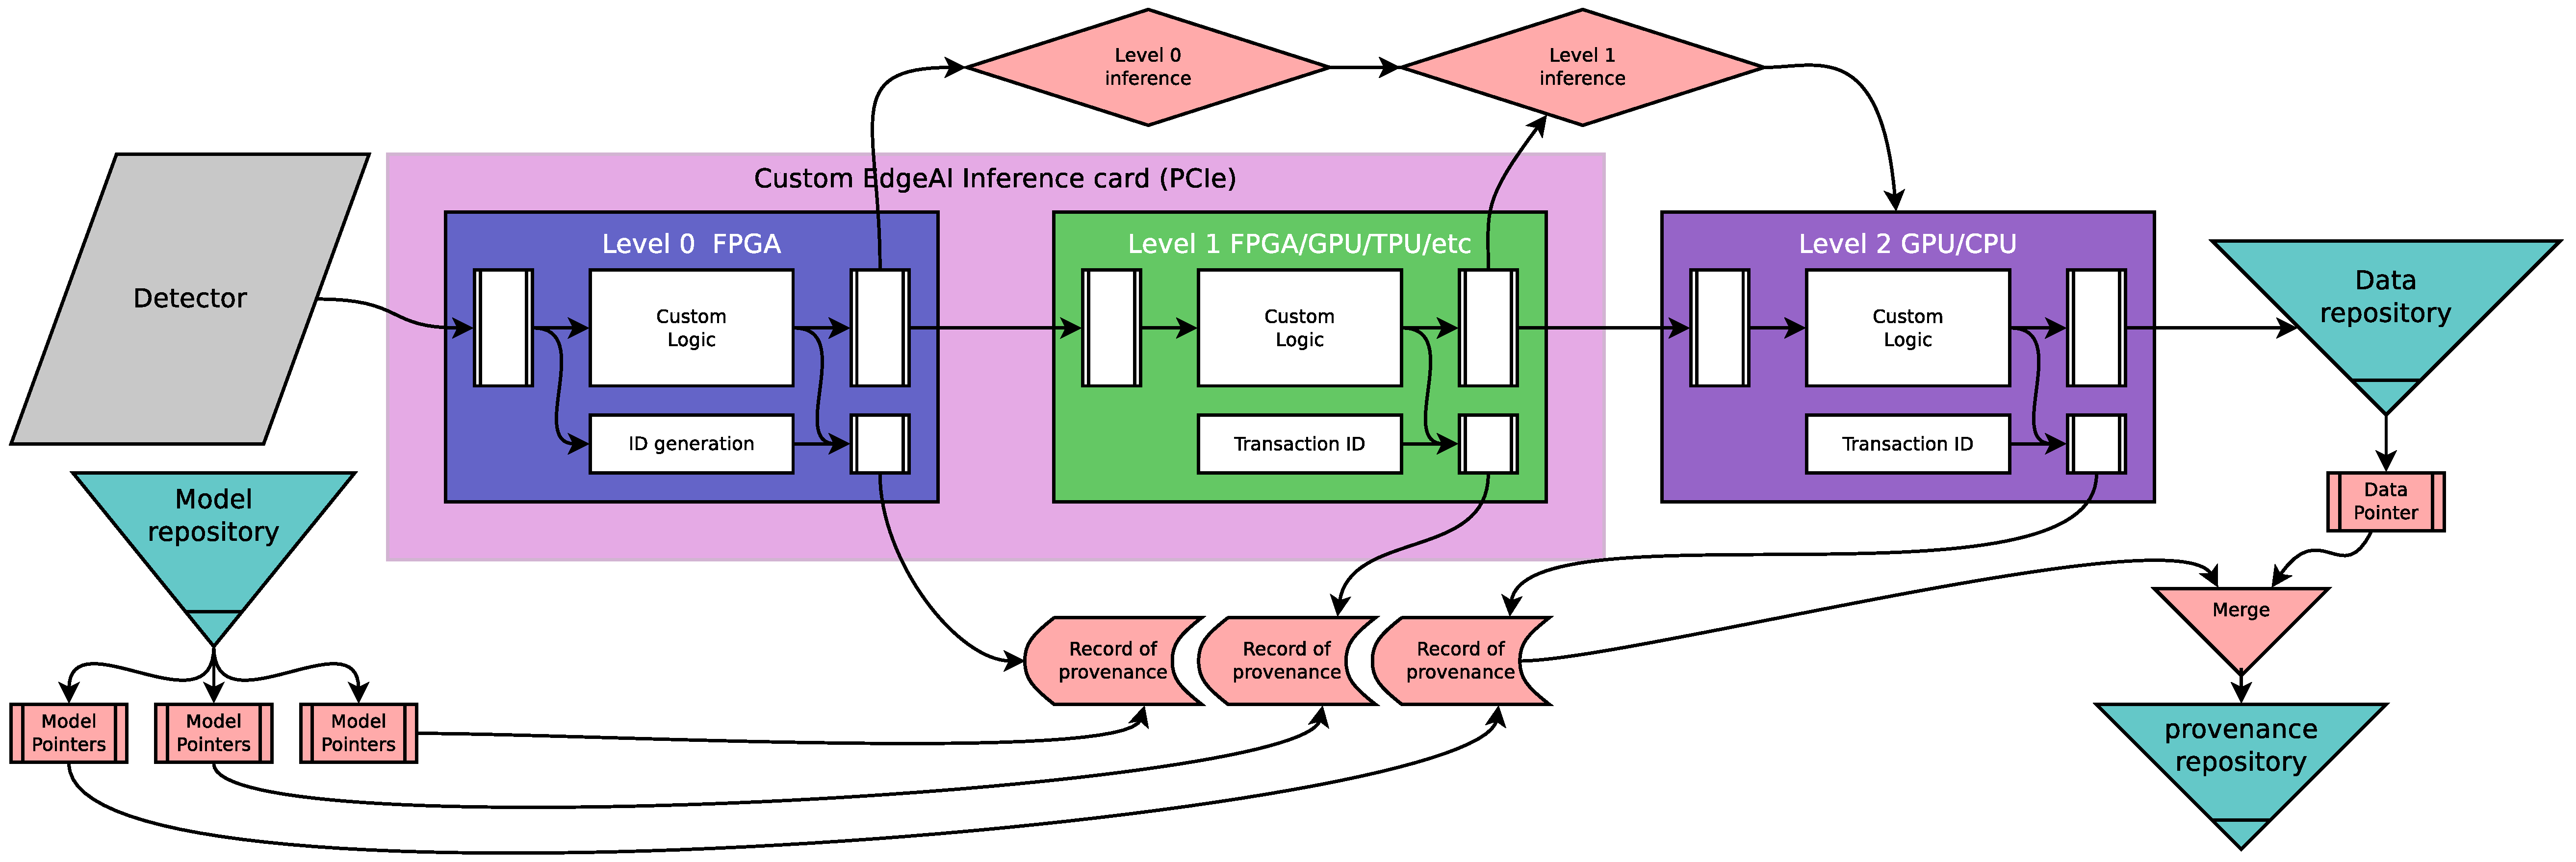
\includegraphics[clip,width=.75\linewidth]{./figs/EdgeFlow.eps}}
	\vspace{-1\baselineskip}
	\caption{
		\label{fig::EdgeFlow}
		Schematic of information flow through heterogeneous hardware with ID generation and provenance tracking.
		}
	\vspace{-1\baselineskip}
\end{figure}

\paragraph{Deliverables}
Ultra-low latency streaming analysis provides actionable information for autonomous feedback control of both the light source and the detector, thus enabling an fully adaptive instrument, source, and analysis pipeline.
The objective of this project is a microsecond scale latency streaming inference optimized for ``batch size=1'' on-sensor FPGA and inference acceleration chip configurations.
The inference engine will optimize data reduction via dynamic data flow routing through a palette of inference accelerators that implement a variety of user-defined domain-specific trained ML model chained in stages. 
The inter-stage control logic will create a state-identifying transaction record that serves as a continual provenance ledger and enables dynamic access and retention control.
This data and algorithm provenance ledger will imbue respective data and algorithms with quantitative metrics that perpetually track derived scientific value.
We will target ultra-high frame rate imaging detectors, including the ePix family of x-ray imaging detectors as well as commercial waveform digitizers and image capture cards.
We will help formulate interface standards for emerging commercial on-detector inference acceleration microchips.

\break

\paragraph{Ryan Coffee (PI): Sr. Staff Scientist, LCLS/PULSE, SLAC National Accelerator Laboratory, coffee@slac.stanford.edu, 650-387-0981. }
\textbf{Graduate and Postdoctoral Advisors: } G.~Gibson (University of Connecticut), P.H.~Bucksbaum (PULSE/Stanford)
\textbf{Graduate Advisees: } Kareem Hegazy (Stanford), Katie Fotion (Cruise Automation), Abdullah Ahmed-Rashed (Brown), Nick Hartmann (Coherent Inc), Mina Bionta (MIT), Doug French (Bettis Atomic Power Laboratory)
\textbf{Postdoctoral Advisees: } Wolfram Helml (U. Dortmund), Markus Ilchen (XFEL), Anton Lindahl (Qamcom), Averell Gatton (SLAC), Audrey Corbeil Therrien (SLAC)
\textbf{Collaborators: }
Ani Aprahamian (Notre Dame), Nora Berrah (U Connecticut), Christoph Bostedt (PSI), Phil Bucksbaum (SLAC), Adrian L Cavalieri (PSI), Martin Centurion (U Nebraska), John Costello (U Dublin), James Cryan (SLAC), Franz-Josef Decker (SLAC), Philip Demekhin (U Kassel), Lou DiMauro (Ohio State U), Hermann A Dürr (Uppsala Univ.), Amir Farbin (UT Arlington), William Fawley (SLAC), Raimund Feifel (U Gothenburg), Thomas Feurer (U Bern), Leszek Frasinski (Imperial College), Alan Fry (SLAC), Andreas Galler (XFEL), Tais Gorkhover (SLAC), Grzhimailo (Lomonosov Moscow State Univ), Jan Grunert (XFEL), Markus Gühr (U Potsdam), Gregor Hartmann (U Kassel), Tony Heinz (SLAC), Wolfram Helml (U. Dortmund), Andrew Hock (Cerebras), Zhirong Huang (SLAC), Markus Ilchen (Euro XFEL), Andreas Junge (Penguin Computing), Nikolai Kabachnik (Lomonosov Moscow State Univ.), Daniel Kane (Mesa Photonics), Reinhard Keinberger (TU Munich), Adam Kirrander (U. Edinburgh), Jeff Koller (Apple), Craig Levin (Stanford), Anton Lindahl (Qamcom), Aaron M Lindenberg (SLAC), Alberto Lutman (SLAC), Jon Marangos (Imperial College), Todd Martínez (Stanford), Serguei Molodtsov (XFEL), Scott Murphy (AMD), Ajay K Nair (Google), Anders Nilsson (U Stockholm), Kunle Olukotun (Stanford), Timor Osipov (NOVA Instruments), Rob Parrish (QCWare), Gregory Penn (LBNL), Rishiraj Pravahan (INQNET), Mohan Rajagopalan (Curious-AI), Daniel Ratner (SLAC), Tor Raubenheimer (SLAC), Dipanwita Ray (KLA-Tencor), Nina Rohringer (U Hamburg), Daniel Rolles (KSU), Arnaud Rouzee (MBI-Berlin), Jan Eric Rubensson (Uppsala U), Artem Rudenko (KSU), Alvaro Sanchez-Gonzalez (DeepMind), Robert Schoenlein (SLAC), Sharon Shwartz (Bar-Ilan U), Klaus Sokolowski-Tinten (Essen Univ.), Mike Styer (Google), Conny Såthe (MAX4 Lund), Ben Taylor (LedgerDomain), Olivier Temam (DeepMind), Thomas Tschentscher (XFEL), Jens Viefhaus (DESY), Xijie Wang (SLAC), Peter Weber (Brown), Chris White (Google) 

\paragraph{Audrey Corbeil Therrien, Banting Research Fellow \& Linac Coherent Light Source (LCLS) Data Systems. }
\textbf{Postdoctoral advisors: } Ryan N. Coffee (SLAC), Jana B. Thayer (SLAC)
\textbf{Graduate advisors: } Serge A. Charlebois (Sherbrooke), R\'{e}jean Fontaine (Sherbrooke), Roger Lecomte (Sherbrooke), Paul Lecoq (CERN), Jean-Francois Pratte (Sherbrooke) 
\textbf{Collaborators: }
Averell Gatton (SLAC), Stefan Gundacker (CERN), William Lemaire (Sherbrooke), Samuel Parent (Sherbrooke), Omar Quijano (SLAC), Marc-Ande\'{e} T\'{e}trault (Sherbrooke, now Harvard Medical School).

\paragraph{Ryan Herbst: Department Head, Electronics Systems, Technology \& Innovation Directorate, Advanced Instrumentation For Research Division. }
\textbf{Collaborators: }
Shiva Abbasazadeh (University of Illinois), David	Abbot	(Jefferson Laboratory), Babek	Abi	(University of Oxford), Nathan	Baltzell	(JLAB), Giles	Barr	(University of Oxford), Marco	Battaglieri	(INFN Genova), Kurt	Biery	(Fermilab), Mariangela	Bondi	(INFN Catania), Sergey	Boyarinov	(JLAB), Stephen	Bueltmann	(ODU), Volker	Burkert	(JLAB), Daniela	Calvo	INFN (Torino), Gabriella	Carini	(Brookhaven), Massimo	Carpinelli	(INFN Sassari), Andrea	Celentano	(INFN Genova), Gabriel	Charles	(ORSAY), William	Cooper	(FNAL), Chris	Cuevas	(JLAB), Annalisa	D'Angelo	(INFN U. Rome), Natalia	Dashyan	(YerPhI), Marzio	De Napoli	(INFN Catania), Alexandre	Deur	(JLAB), Raffaella	DeVita	(INFN Genova), Raphaël	Dupre	(ORSAY), Hovanes	Egiyan	(JLAB), Latifa	Elouadrhiri	(JLAB), Rouven	Essig	(Stony Brook U.), Vitaliy	Fadeyev	(UCSC), Alessandra	Filippi	(INFN Torino), Arne	Freyberger	(JLAB), Michel	Garçon	(CEA-Saclay), Nerses	Gevorgyan	(YerPhI), Francois-Xavier	(Girod	JLAB), Keith	Griffioen	(W\&M), Michel	Guidal	(ORSAY), Maurik	Holtrop	(UNH), Greg	Kalicy	(ODU), Mahbub	Khandaker	(Idaho U.), Emanuele	Leonora	(INFN Catania), Luca	Marsicano	(INFN Genova), Kyle	McCarty	(UNH), Bryan	McKinnon	(Glasgow U.), Carlos	Munoz-Camacho	(ORSAY), Silvia	Niccolai	(ORSAY), Kurtis	Nishimura	(University Of Hawaii), Michail	Osipenko	(INFN Genova), Rafayel	Paremuzyan	(UNH), Nunzio	Randazzo	(INFN Catania), Ben	Raydo	(JLAB), Alessandro	Rizzo	(INFN U. Rome), Youri	Sharabian	(JLAB), Gabriele	Simi	(INFN Padova), Valeria	Sipala	(INFN Sassari), Stepan	Stepanyan	(JLAB), David	Strom	(University Of Oregon), Lauren	Thompkins	(Stanford), Sho	Uemura	(Los Alamos), Maurizio	Ungaro	(JLAB), Holly	Vance	(JLAB), Gary	Varner	(University Of Hawaii), Hakop	Voskanyan	(YerPhI), Andrew	White	(University Of Texas, Arlington), Bradley	Yale	(UNH)


\paragraph{Ben Taylor, Founder and CEO, LedgerDomain, LLC.  }
\textbf{Graduate advisor: } William H Orme-Johnson.
\textbf{Collaborators: }
Perry Shieh (UCLA), Josenor deJesus (UCLA) and William Chien (UCLA).

\paragraph{Omar Quijano, Department Head, Linac Coherent Light Source (LCLS) IT/Networking. }
\textbf{Graduate Advisor: } Nikos Mourtos
\textbf{Collaborators: }
Patrick H Reisenthal, Daniel J. Lesieutre, Michael R. Mendenhall, Harrison S. Y. Chou, Joel Tambaoan, Ivan Tan, Namgyal Tesur, Ian Dupzyk, Linda Contreras, Sean Montgomery.

\paragraph{Matt Feldman, Graduate Fellow, Stanford Computer Science \& Developer SambaNova Systems. }
\textbf{Graduate advisor: } Kunle Olukotun.
\textbf{Colaborators: }
David Koeplinger (Stanford), Raghu Prabhakar (Stanford), Yaqi Zhang (Stanford), Stefan Hadjis (Stanford), Ruben Fiszel (EPFL Switzerland), Tian Zhao (Stanford), Luigi Nardi (Stanford), Ardavan Pedram (Stanford), Christos Kozyrakis (Stanford)

\paragraph{Angelo Dragone (not funded), Department Head, Integrated Circuits, Technology \& Innovation Directorate, Advanced Instrumentation For Research Division. }

\paragraph{Jana Thayer (not funded), Department Head, Linac Coherent Light Source (LCLS) Data Systems. }

\bibliography{whitepaper.bib}

\end{document}

